% rf_interfaces.tex — ONE source, ONE rendered SVG (rf_interfaces.svg), embedded in
% ../rfdc/index.md under "## Interfaces".
%
% The claim: ONE module carries BOTH directions, and the two sides are different kinds of port.
% Your logic is on the left because that is the side you write; the RF environment is on the right
% because it is the side you do not.  RX flows right-to-left and TX left-to-right, which is why the
% converter cannot be two blocks: the two grids share a time origin that belongs to the module.
%
% Distinct from rf_domains.tex, which asserts a REPRESENTATION claim (sample blocks vs packed
% words).  This one asserts an INTERFACE claim: four endpoints, two clock domains.
%
% Render: bash render.sh   (MiKTeX pdflatex -> PDF -> dvisvgm --pdf -> SVG)
\documentclass[tikz,border=4pt]{standalone}
\usepackage{tikz}
\usetikzlibrary{arrows.meta,positioning,calc,fit,backgrounds}

% NYU palette.  Violet is the house colour and marks everything we MODEL; the RF environment is
% deliberately grey because it is the boundary whose far side we refuse to model at RTL.  The
% converter is solid violet with reversed text so the eye lands on the boundary first.
\definecolor{nyuviolet}{HTML}{57068C}
\definecolor{nyuultra}{HTML}{330662}
\definecolor{nyupale}{HTML}{EFE6F5}
\definecolor{nyumid}{HTML}{8A5FB0}
\definecolor{envfill}{HTML}{F1EFF3}
\definecolor{envline}{HTML}{6E6A73}
\definecolor{inkgray}{HTML}{444444}

\begin{document}
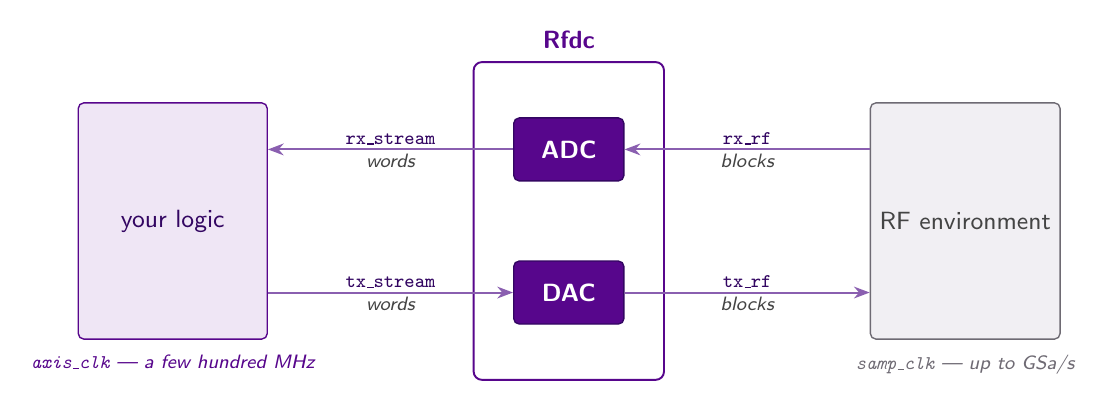
\begin{tikzpicture}[
  font=\sffamily\small,
  fab/.style  = {draw=nyuviolet, line width=0.5pt, fill=nyupale, rounded corners=2pt,
                 minimum width=24mm, minimum height=30mm, text=nyuultra},
  env/.style  = {draw=envline, line width=0.5pt, fill=envfill, rounded corners=2pt,
                 minimum width=24mm, minimum height=30mm, text=inkgray},
  core/.style = {draw=nyuultra, line width=0.5pt, fill=nyuviolet, rounded corners=2pt,
                 minimum width=14mm, minimum height=8mm, text=white, font=\sffamily\small\bfseries},
  box/.style  = {draw=nyuviolet, line width=0.7pt, fill=white, rounded corners=3pt},
  ln/.style   = {-{Stealth[length=2mm]}, draw=nyumid, line width=0.7pt},
  lbl/.style  = {font=\sffamily\scriptsize, text=nyuultra, inner sep=1.4pt},
  sub/.style  = {font=\sffamily\scriptsize\itshape, text=inkgray, inner sep=1.2pt},
]

% --- the converter, and the two paths inside it --------------------------------------------------
\node[core] (adc) {ADC};
\node[core, below=10mm of adc] (dac) {DAC};
\begin{scope}[on background layer]
  \node[box, fit=(adc)(dac), inner xsep=5mm, inner ysep=7mm] (rfdc) {};
\end{scope}
\node[lbl, font=\sffamily\small\bfseries, text=nyuviolet, above=1mm of rfdc.north] {Rfdc};

% --- the two sides -------------------------------------------------------------------------------
\node[fab, left=26mm of rfdc]  (dut) {your logic};
\node[env, right=26mm of rfdc] (env) {RF environment};

% --- RX: environment -> ADC -> your logic (right to left) ----------------------------------------
\draw[ln] (env.west |- adc) -- node[lbl, above] {\texttt{rx\_rf}}
                               node[sub, below] {blocks} (adc.east);
\draw[ln] (adc.west) -- node[lbl, above] {\texttt{rx\_stream}}
                        node[sub, below] {words} (dut.east |- adc);

% --- TX: your logic -> DAC -> environment (left to right) ----------------------------------------
\draw[ln] (dut.east |- dac) -- node[lbl, above] {\texttt{tx\_stream}}
                               node[sub, below] {words} (dac.west);
\draw[ln] (dac.east) -- node[lbl, above] {\texttt{tx\_rf}}
                        node[sub, below] {blocks} (env.west |- dac);

% --- the two clock domains -----------------------------------------------------------------------
\node[sub, below=1.5mm of dut.south, text=nyuviolet]
  {\texttt{axis\_clk} --- a few hundred MHz};
\node[sub, below=1.5mm of env.south, text=envline]
  {\texttt{samp\_clk} --- up to GSa/s};

\end{tikzpicture}
\end{document}
